\documentclass[11pt,a4paper]{article}

\usepackage[T1]{fontenc}
\usepackage{lmodern}
\usepackage[a4paper,margin=2.2cm]{geometry}
\usepackage{amsmath,amssymb}
\usepackage{graphicx}
\usepackage{booktabs}
\usepackage{siunitx}
\usepackage{caption}
\usepackage{tikz}
\usepackage{pgfplots}
\pgfplotsset{compat=1.16}
\usetikzlibrary{arrows.meta,calc,decorations.pathreplacing}
\usepackage[colorlinks=true,linkcolor=blue!50!black,citecolor=blue!50!black,urlcolor=blue!50!black]{hyperref}

\captionsetup{font=small,labelfont=bf}
\setlength{\parskip}{4pt}
\setlength{\parindent}{0pt}

\newcommand{\FP}{Fabry-P\'erot}
\newcommand{\FSR}{\Delta\nu_{\mathrm{FSR}}}
\newcommand{\Fin}{\mathcal{F}}
\newcommand{\ii}{\mathrm{i}}

\title{\textbf{Fabry-P\'erot Interferometer:\\ Modes and Stability of the Cavity}}
\author{
	Mohammed Al-Twaity\\
	Husni Naufal Zuhdi\\
	Khalil Assaf
}
\date{\today}

\begin{document}
	
	\maketitle
	
	\begin{abstract}
		\noindent
		The \FP{} interferometer, two parallel partially reflecting surfaces facing each other, is one of the simplest and most widely used devices in optics. It is a high-resolution spectral analyser when used passively, and it is also the basic geometry of almost every laser resonator. This report reviews the principle of multiple-beam interference in a \FP{} etalon (Airy function, free spectral range, finesse and resolving power) and shows how the same structure acts as a resonator for a laser. We then discuss the longitudinal and transverse modes of an optical cavity, derive the stability condition $0\le g_1g_2\le 1$ from ray-transfer matrices, and analyse the Gaussian beam supported by a stable cavity. Finally, we discuss how the cavity configuration influences laser performance (beam size, mode content, alignment sensitivity) and illustrate the results with a helium-neon laser, a semiconductor laser diode, and other applications.
	\end{abstract}
	
	
	%==========================================================================
	\section{Definition of a \FP{} Interferometer and Optical Cavity}
	%==========================================================================
	
	A \textbf{\FP{} interferometer} (FPI) is a device consists of two parallel, with partially reflecting surfaces that separated by a distance $d$. Each surfaces can be coated with a transparent plate, which usually called a \FP{} etalon. The device was introduced bye Charles Fabry and Alfred P\'erot in 1899 as a high resolution spectroscopy tool \cite{FabryPerot1899}. The light entering the gap is reflected back and forth many times, and then a small fraction of it leaves through the second surface at every interaction. These many transmitted beams are copies of the incident wave with a delay of constant optical path and they interfere with each other \cite{BornWolf, Hecht, Vaughan}.
	
	An \textbf{optical cavity} (or optical resonator) is a more general concept: an arrangement of reflecting elements that traps light so that it circulates along a closed path and self-reproduce each trips. The \FP{} cavity, formed by two mirrors facing each other, is one of the example of a \emph{standing-wave} resonator. The mirrors could be flat or curved. A flat-flat pair is the classical \FP{} etalon; a pair of curved mirrors forms the spherical-mirror resonator used in most lasers \cite{Siegman,Svelto,SalehTeich}.
	
	The same physical structure plays two different roles:
	\begin{itemize}
		\item \textbf{Passive role.} An external light source is analysed or filtered. The cavity transmits only certain frequencies, so it acts as a spectrometer, a narrow-band filter or a frequency reference.
		\item \textbf{Active role.} A gain medium is placed inside the cavity. The mirrors provide the optical feedback that turns an amplifier into an oscillator, and the cavity also decides which frequencies and which spatial patterns can oscillate. This was recognised at the very beginning of laser physics \cite{SchawlowTownes1958}, and the first laser, the ruby laser of 1960, used a pair of parallel coated faces of the crystal as its \FP{} cavity \cite{Maiman1960}.
	\end{itemize}
	
	The parameters that describe the cavity throughout this report are the mirror power reflectivities $R_1$ and $R_2$ (or a common value $R$), the mirror spacing $L$ (written $d$ for an etalon), the refractive index $n$ of the medium between the mirrors, and, for curved mirrors, the radii of curvature $R_{c1}$ and $R_{c2}$.
	
	%==========================================================================
	\section{Principle of the \FP{} Interferometer}
	%==========================================================================
	
	\subsection{Optical path difference between successive beams}
	
	Consider a plane wave incident on a plate of thickness $d$ and refractive index $n$, surrounded by a medium of index $n_0$. Let $\theta$ be the angle \emph{inside} the plate, related to the external angle $\theta_0$ by Snell's law, $n_0\sin\theta_0=n\sin\theta$. Fig.~\ref{fig:opd} follows one ray that enters at $A$, reaches the second surface at $B$, where part of it is transmitted (ray~1) and part is reflected back to $C$ on the first surface. At $C$ it is reflected again and reaches the second surface at $D$, where it is transmitted (ray~2). Rays 1 and 2 are parallel and are brought together by a lens, so their phase difference is set by the difference in optical path up to a common wavefront (the dashed line $DF$ perpendicular to the rays).
	
	
	\begin{figure}[ht]
		\centering
		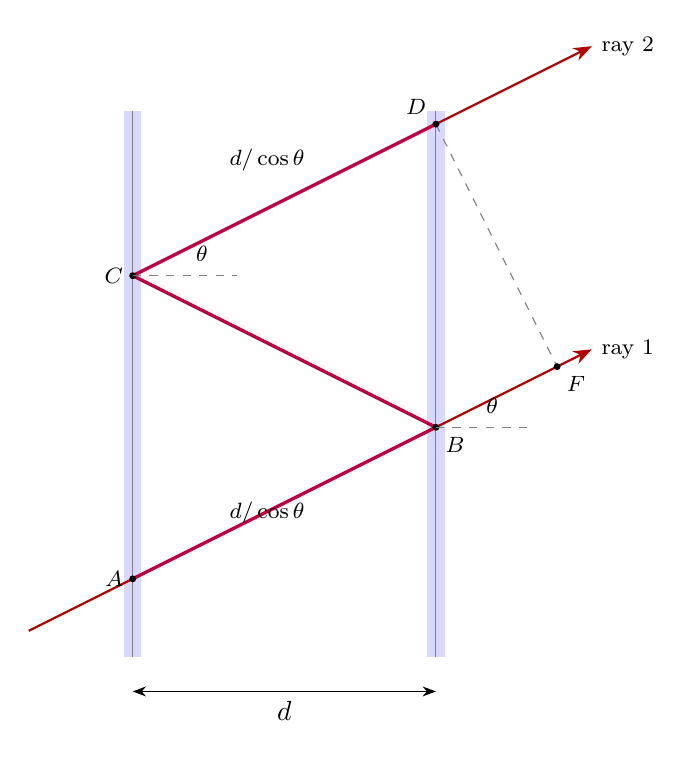
\begin{tikzpicture}[scale=1.1,>=Stealth]
			\fill[blue!15] (-0.1,-0.9) rectangle (0.1,5.4);
			\fill[blue!15] (3.4,-0.9) rectangle (3.6,5.4);
			\draw[gray] (0,-0.9) -- (0,5.4);
			\draw[gray] (3.5,-0.9) -- (3.5,5.4);
			% points: A(0,0) B(3.5,1.75) C(0,3.5) D(3.5,5.25)
			\draw[red!70!black,thick] (-1.2,-0.6) -- (0,0);
			\draw[red!70!black,very thick,purple] (0,0) -- (3.5,1.75) -- (0,3.5) -- (3.5,5.25);
			\draw[->,red!70!black,thick] (3.5,1.75) -- (5.3,2.65);
			\draw[->,red!70!black,thick] (3.5,5.25) -- (5.3,6.15);
			\node[right,font=\footnotesize] at (5.3,2.65) {ray 1};
			\node[right,font=\footnotesize] at (5.3,6.15) {ray 2};
			% wavefront through D, foot F on ray 1
			\draw[dashed,gray] (3.5,5.25) -- (4.9,2.45);
			\fill (4.9,2.45) circle (0.04) node[below right,font=\footnotesize] {$F$};
			\fill (0,0) circle (0.04) node[left,font=\footnotesize] {$A$};
			\fill (3.5,1.75) circle (0.04) node[below right,font=\footnotesize] {$B$};
			\fill (0,3.5) circle (0.04) node[left,font=\footnotesize] {$C$};
			\fill (3.5,5.25) circle (0.04) node[above left,font=\footnotesize] {$D$};
			% normal and angle
			\draw[dashed,gray] (3.5,1.75) -- (4.6,1.75);
			\draw[dashed,gray] (0,3.5) -- (1.2,3.5);
			\node[font=\footnotesize] at (4.15,2.0) {$\theta$};
			\node[font=\footnotesize] at (0.8,3.75) {$\theta$};
			% labels
			\node[font=\footnotesize,above] at (1.55,4.6) {$d/\cos\theta$};
			\node[font=\footnotesize,below] at (1.55,1.0) {$d/\cos\theta$};
			\draw[<->] (0,-1.3) -- (3.5,-1.3);
			\node[below] at (1.75,-1.3) {$d$};
		\end{tikzpicture}
		\caption{Geometry for the optical path difference of two successive transmitted beams. The extra path of ray~2 is $BC+CD$ inside the plate, minus the length $BF$ that ray~1 travels to reach the common wavefront $DF$.}
		\label{fig:opd}
	\end{figure}
	
	From the geometry, $BC=CD=d/\cos\theta$, $BD=2d\tan\theta$ and $BF=BD\sin\theta$. The optical path difference is therefore
	\begin{align}
		\Delta\mathrm{OPL} &= n\left(BC+CD-BF\right)=n\left(\frac{2d}{\cos\theta}-2d\tan\theta\sin\theta\right)=2nd\cos\theta .
		\label{eq:opl}
	\end{align}
	The same result is obtained by projecting the segments onto the wavefront, which gives the equivalent form
	\begin{equation}
		\Delta\mathrm{OPL}=n\left[\frac{d}{\cos\theta}\cos2\theta+\frac{d}{\cos\theta}\right]
		=nd\,\frac{2\cos^2\theta-1+1}{\cos\theta}=2nd\cos\theta .
	\end{equation}
	The corresponding phase difference between adjacent beams is
	\begin{equation}
		\delta=\frac{2\pi}{\lambda}\,\Delta\mathrm{OPL}+\varphi=\frac{4\pi nd\cos\theta}{\lambda}+\varphi,
		\label{eq:delta}
	\end{equation}
	where $\varphi$ is the total phase change on the two internal reflections ($\varphi/2$ per reflection). Without it, $\delta$ is the purely geometric phase $4\pi nd\cos\theta/\lambda$.
	
	
	
	\paragraph{Can the reflection phase be ignored?} Usually yes, as an approximation. If $\varphi$ is the same for all wavelengths of interest it only adds a constant to $\delta$, so the resonance condition $\delta=2\pi m$ becomes $2nd\cos\theta=(m-\varphi/2\pi)\lambda$. The peaks shift slightly (the plate behaves as if its thickness were changed by a small constant), but their spacing, shape and finesse are unchanged. The phase must be kept when the absolute spacing is to be measured, or when the coating is dispersive, so that $\varphi$ varies noticeably across the wavelength range \cite{BornWolf,Vaughan}.
	
	\subsection{Amplitude and power coefficients}
	
	Let $r$ and $t$ be the amplitude reflection and transmission coefficients for a wave going into the plate, and $r'$ and $t'$ those for a wave leaving it (Fig.~\ref{fig:etalon}). For a lossless interface the Stokes relations give
	\begin{equation}
		r'=-r, \qquad tt'=1-r^2 .
	\end{equation}
	The \emph{power} (irradiance) coefficients follow from the Fresnel equations,
	\begin{equation}
		R=\frac{P_r}{P_i}=r^2, \qquad T=\frac{P_t}{P_i}=\frac{n_2\cos\theta_t}{n_1\cos\theta_i}\,t^2 .
		\label{eq:RT}
	\end{equation}
	The power transmission is therefore \emph{not} equal to $t^2$: the factor $n_2\cos\theta_t/n_1\cos\theta_i$ accounts for the change of beam cross-section and wave speed at the surface. For a plate, the beam crosses a front surface (air to glass, ratio $n_g/1$) and a back surface (glass to air, ratio $1/n_g$), and these factors cancel in the product:
	\begin{equation}
		T_{\mathrm{front}}T_{\mathrm{back}}=\left(\frac{n_g}{1}\,t^2\right)\left(\frac{1}{n_g}\,t'^2\right)=(tt')^2 .
	\end{equation}
	For two identical lossless surfaces $T_{\mathrm{front}}=T_{\mathrm{back}}=T=1-R$, so $T_{\mathrm{front}}T_{\mathrm{back}}=T^2=(1-R)^2$, and this is the factor that appears in the transmitted irradiance below.
	
	\subsection{Sum of the transmitted beams}
	
	Each transmitted beam has crossed the plate once more than the previous one, picking up a factor $r'^2e^{\ii\delta}=R\,e^{\ii\delta}$ (two internal reflections and one extra round-trip phase), as indicated in Fig.~\ref{fig:etalon}. The total transmitted field is the geometric series
	\begin{equation}
		E_t = E_0\,tt'\sum_{k=0}^{\infty}\left(R\,e^{\ii\delta}\right)^k = \frac{E_0\,tt'}{1-R\,e^{\ii\delta}} .
	\end{equation}
	
	\begin{figure}[ht]
		\centering
		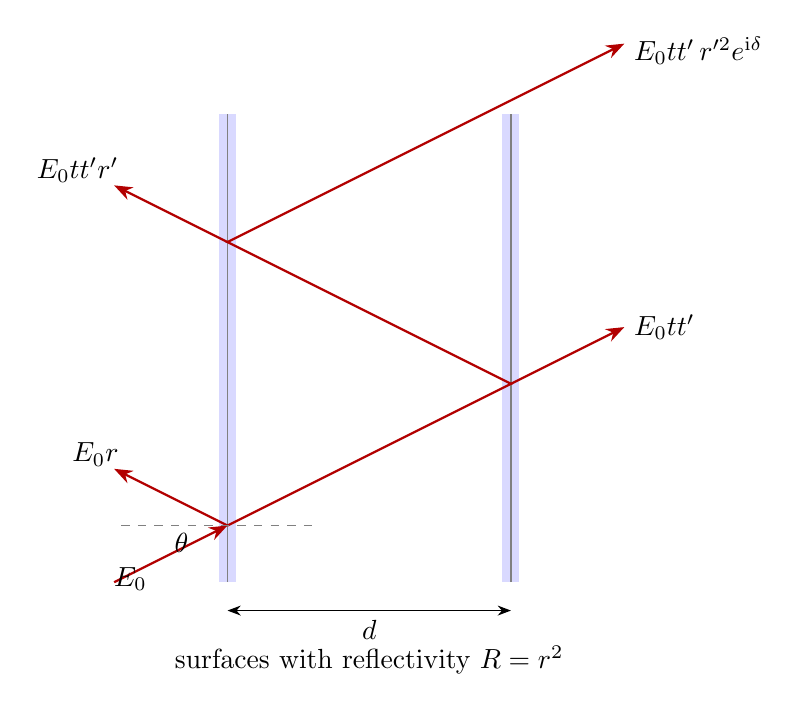
\begin{tikzpicture}[scale=0.9,>=Stealth]
			\fill[blue!15] (-0.12,-0.8) rectangle (0.12,5.8);
			\fill[blue!15] (3.88,-0.8) rectangle (4.12,5.8);
			\draw[gray] (0,-0.8) -- (0,5.8);
			\draw[gray] (4,-0.8) -- (4,5.8);
			\draw[->,red!70!black,thick] (-1.6,-0.8) -- (0,0);
			\node[below left] at (-1.0,-0.45) {$E_0$};
			\draw[->,red!70!black,thick] (0,0) -- (-1.6,0.8);
			\node[above left] at (-1.4,0.7) {$E_0r$};
			\draw[red!70!black,thick] (0,0) -- (4,2) -- (0,4) -- (4,6);
			\draw[->,red!70!black,thick] (0,4) -- (-1.6,4.8);
			\node[above left] at (-1.4,4.7) {$E_0tt'r'$};
			\draw[->,red!70!black,thick] (4,2) -- (5.6,2.8);
			\node[right] at (5.6,2.8) {$E_0tt'$};
			\draw[->,red!70!black,thick] (4,6) -- (5.6,6.8);
			\node[right] at (5.6,6.7) {$E_0tt'\,r'^{2}e^{\ii\delta}$};
			\draw[<->] (0,-1.2) -- (4,-1.2);
			\node[below] at (2,-1.2) {$d$};
			\node at (2,-1.9) {surfaces with reflectivity $R=r^2$};
			\draw[dashed,gray] (-1.5,0) -- (1.2,0);
			\node at (-0.65,-0.25) {$\theta$};
		\end{tikzpicture}
		\caption{Multiple-beam interference in a \FP{} etalon (schematic). Each successive transmitted beam is delayed by the round-trip phase $\delta$ and attenuated by $R=r^2$ relative to the previous one. The first transmitted beam has amplitude $E_0tt'$.}
		\label{fig:etalon}
	\end{figure}
	
	\subsection{Transmitted irradiance and the Airy function}
	
	The irradiance is proportional to $|E_t|^2$. Using $|tt'|^2=T_{\mathrm{front}}T_{\mathrm{back}}=T^2$,
	\begin{equation}
		I_t=I_0\,\frac{T^2}{\left|1-R\,e^{\ii\delta}\right|^2}.
	\end{equation}
	The denominator is expanded using $|z|^2=zz^*$ and $\cos\delta=(e^{\ii\delta}+e^{-\ii\delta})/2$:
	\begin{align}
		\left|1-R\,e^{\ii\delta}\right|^2 &=(1-Re^{\ii\delta})(1-Re^{-\ii\delta})
		=1+R^2-2R\cos\delta \nonumber\\
		&=(1-R)^2+2R(1-\cos\delta)=(1-R)^2+4R\sin^2\!\left(\frac{\delta}{2}\right),
		\label{eq:denom}
	\end{align}
	where the last step uses $1-\cos\delta=2\sin^2(\delta/2)$. Inserting this and factoring out $(1-R)^2$ gives the \textbf{Airy function}
	\begin{equation}
		\frac{I_t}{I_0}=\frac{T^2}{(1-R)^2}\;\frac{1}{1+F\sin^2(\delta/2)},\qquad F=\frac{4R}{(1-R)^2},
		\label{eq:airy}
	\end{equation}
	where $F$ is the \emph{coefficient of finesse} \cite{BornWolf,Hecht,SalehTeich}. The prefactor $T^2/(1-R)^2$ is the maximum transmission $I_{t,\max}/I_0$. For a lossless etalon $T=1-R$, so it equals~1 and every wavelength satisfying the resonance condition is transmitted completely. If the surfaces absorb or scatter a fraction $A$ of the power, then $T=1-R-A$ and the peak transmission falls to $[1-A/(1-R)]^2$; the shape of the resonance is unchanged.
	
	\subsection{Resonance condition, free spectral range, finesse}
	
	The transmission is maximal ($I_t=I_0$) when $\delta=2\pi m$ with $m$ an integer, that is,
	\begin{equation}
		2nd\cos\theta_t = m\lambda ,
		\label{eq:resonance}
	\end{equation}
	which is the condition $2d\cos\alpha=m\lambda$ commonly quoted for an air-spaced device (with the reflection phase $\varphi$ included, $m$ is replaced by $m-\varphi/2\pi$). It means that the round trip contains an integer number of wavelengths, so all transmitted beams are in phase. Between two peaks the transmission falls to a minimum of $I_{\min}/I_0=[(1-R)/(1+R)]^2$ (lossless case). For normal incidence, the spacing between adjacent resonances in frequency is the \textbf{free spectral range} (FSR),
	\begin{equation}
		\FSR = \frac{c}{2nd}, \qquad \Delta\lambda_{\mathrm{FSR}}\simeq\frac{\lambda^2}{2nd}.
		\label{eq:fsr}
	\end{equation}
	The full width at half maximum of a transmission peak, in phase, is $\Delta\delta\approx 4/\sqrt F$ for $R$ not too small. The ratio of the FSR to the peak width defines the \textbf{finesse},
	\begin{equation}
		\Fin = \frac{\FSR}{\delta\nu_{1/2}} = \frac{\pi\sqrt F}{2} = \frac{\pi\sqrt R}{1-R}.
		\label{eq:finesse}
	\end{equation}
	The finesse depends only on the mirror quality, while the FSR depends only on the spacing. Fig.~\ref{fig:airy} shows how increasing $R$ narrows the peaks and darkens the gaps between them.
	
	\begin{figure}[ht]
		\centering
		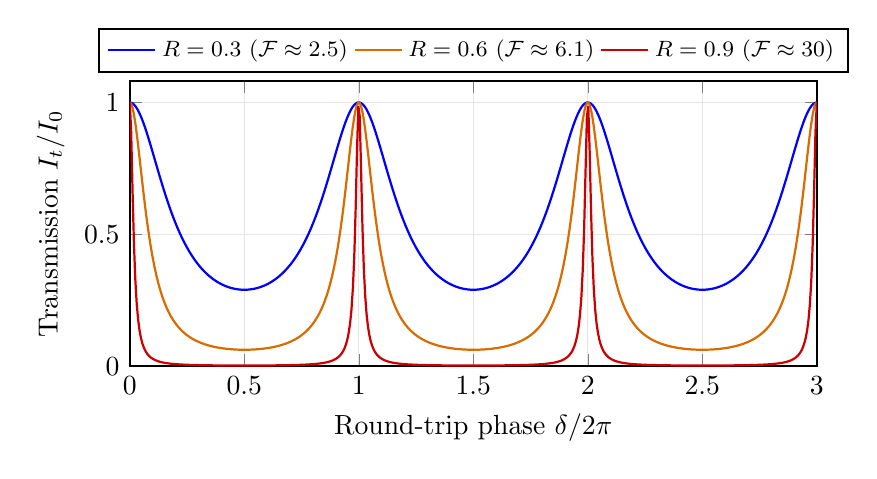
\begin{tikzpicture}
			\begin{axis}[
				width=0.85\textwidth, height=5.2cm,
				xlabel={Round-trip phase $\delta/2\pi$},
				ylabel={Transmission $I_t/I_0$},
				xmin=0, xmax=3, ymin=0, ymax=1.08,
				legend style={font=\footnotesize, at={(0.5,1.03)}, anchor=south, legend columns=3},
				samples=500, no markers, thick, grid=both, grid style={gray!20}]
				\addplot[blue,domain=0:3]{1/(1+2.449*(sin(180*x))^2)};
				\addplot[orange!85!black,domain=0:3]{1/(1+15*(sin(180*x))^2)};
				\addplot[red!80!black,domain=0:3]{1/(1+360*(sin(180*x))^2)};
				\legend{$R=0.3\ (\Fin\approx2.5)$, $R=0.6\ (\Fin\approx6.1)$, $R=0.9\ (\Fin\approx30)$}
			\end{axis}
		\end{tikzpicture}
		\caption{Airy transmission function, Eq.~\eqref{eq:airy}, of a lossless \FP{} etalon for three mirror reflectivities. The distance between neighbouring peaks is one free spectral range.}
		\label{fig:airy}
	\end{figure}
	
	\subsection{Resolving power and tuning}
	
	At resonance, the order is $m=2nd/\lambda$ (for normal incidence), and the \textbf{chromatic resolving power} is approximately
	\begin{equation}
		\frac{\lambda}{\delta\lambda_{\min}} \approx m\,\Fin = \frac{2nd}{\lambda}\,\frac{\pi\sqrt R}{1-R}.
	\end{equation}
	This is why an interferometer with a modest spacing can resolve lines that a prism or grating spectrometer of similar size cannot: the effective number of interfering beams is of order $\Fin$, which plays the role of the number of slits in a grating \cite{Vaughan,Hernandez}.
	
	\emph{Numerical example.} A fused-silica etalon of thickness $d=\SI{1}{mm}$ ($n\approx1.45$) with $R=0.9$ has $\FSR=c/(2nd)\approx\SI{103}{GHz}$, $\Fin\approx30$, a peak width of about $\SI{3.5}{GHz}$, and, at $\lambda=\SI{632.8}{nm}$, an order $m\approx4.6\times10^{3}$ and a resolving power of roughly $1.4\times10^{5}$.
	
	The resonance condition \eqref{eq:resonance} can be tuned by changing $d$ (piezo scanning), the angle $\theta$ (tilting), or the index $n$ (temperature or gas pressure). A scanning interferometer, in which $d$ is swept while a photodiode records the transmitted power, therefore produces the spectrum of the incident light as a series of peaks repeated every FSR. With a lens, the angular dependence in \eqref{eq:resonance} creates the concentric ring pattern seen on a screen, with the highest orders near the centre \cite{Hecht}.
	
	%==========================================================================
	\section{\FP{} Cavity as a Laser Resonator}
	%==========================================================================
	
	A laser consists of three ingredients: a gain medium, a pump that inverts its population, and \emph{optical feedback}. The \FP{} cavity provides the feedback. A single pass through a gain medium of length $\ell$ amplifies the intensity only by a factor $e^{g\ell}$, which is small in most lasers. By placing the medium between two mirrors the light passes through it many times, so even a weak gain can build up an intense field \cite{Siegman,Svelto,Milonni}. In addition, the cavity selects which frequencies and which transverse patterns are amplified, giving the laser its narrow linewidth and its well-defined beam.
	
	\begin{figure}[ht]
		\centering
		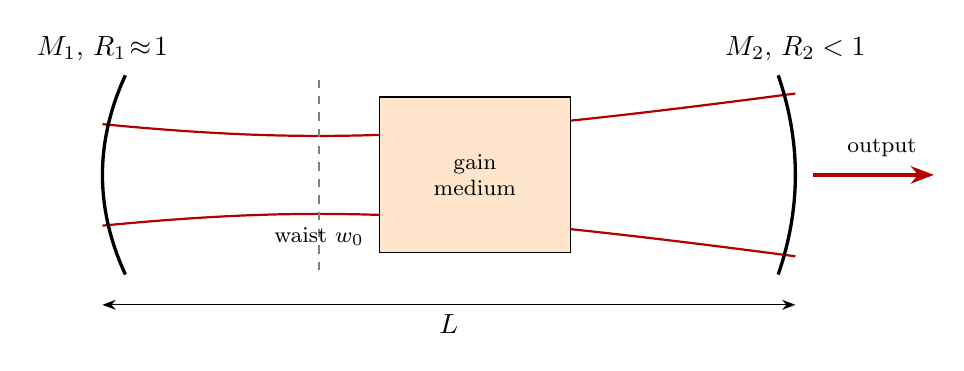
\begin{tikzpicture}[>=Stealth,scale=1.1]
			% envelope
			\draw[red!70!black,thick,domain=0:8,smooth,variable=\x]
			plot ({\x},{0.45*sqrt(1+((\x-2.5)/3)*((\x-2.5)/3))});
			\draw[red!70!black,thick,domain=0:8,smooth,variable=\x]
			plot ({\x},{-0.45*sqrt(1+((\x-2.5)/3)*((\x-2.5)/3))});
			% gain medium
			\draw[fill=orange!20] (3.2,-0.9) rectangle (5.4,0.9);
			\node[align=center,font=\footnotesize] at (4.3,0) {gain\\medium};
			% mirrors
			\draw[very thick,domain=-1.15:1.15,smooth,variable=\y] plot ({0.2*\y*\y},{\y});
			\draw[very thick,domain=-1.15:1.15,smooth,variable=\y] plot ({8-0.15*\y*\y},{\y});
			\node[above] at (0,1.2) {$M_1$, $R_1\!\approx\!1$};
			\node[above] at (8,1.2) {$M_2$, $R_2<1$};
			% output
			\draw[->,very thick,red!70!black] (8.2,0) -- (9.6,0);
			\node[above,font=\footnotesize] at (9.0,0.1) {output};
			% length
			\draw[<->] (0,-1.5) -- (8,-1.5);
			\node[below] at (4,-1.5) {$L$};
			% waist marker
			\draw[dashed,gray] (2.5,-1.1) -- (2.5,1.1);
			\node[below,font=\footnotesize] at (2.5,-0.5) {waist $w_0$};
		\end{tikzpicture}
		\caption{A two-mirror laser resonator. The mirrors define a Gaussian beam of waist $w_0$ whose wavefront curvature matches the mirror radii (Sec.~\ref{sec:stability}). Mirror $M_2$ is partially transmitting and works as the output coupler.}
		\label{fig:lasercavity}
	\end{figure}
	
	\subsection{Threshold condition}
	
	For steady-state oscillation the field must reproduce itself, in amplitude and phase, after one round trip. Let $g$ be the (intensity) gain coefficient of the medium, $\alpha_s$ the distributed loss from scattering and absorption in the cavity, and $R_1$, $R_2$ the mirror reflectivities. The amplitude condition is
	\begin{equation}
		R_1R_2\,e^{2(g-\alpha_s)L}=1
		\quad\Longrightarrow\quad
		g_{\mathrm{th}}=\alpha_s+\frac{1}{2L}\ln\frac{1}{R_1R_2}.
		\label{eq:threshold}
	\end{equation}
	The second term is the \emph{mirror loss}, and it is the price paid for letting the light escape through $M_2$. The lifetime of a photon in the cavity is
	\begin{equation}
		\tau_c = \frac{2nL/c}{\mathcal{L}_{\mathrm{rt}}}, \qquad \mathcal{L}_{\mathrm{rt}}\simeq 2\alpha_sL+\ln\frac{1}{R_1R_2},
	\end{equation}
	that is, the round-trip time divided by the fractional loss per round trip, and the corresponding cold-cavity linewidth is $\delta\nu_c=1/(2\pi\tau_c)$. For two mirrors of equal reflectivity $R\to1$ and no other loss, this expression is identical to $\FSR/\Fin$ from Eq.~\eqref{eq:finesse}. The laser cavity is therefore the \emph{same} \FP{} resonator as the passive interferometer, and the finesse is just another way of expressing the cavity loss \cite{Siegman,Svelto}.
	
	The \emph{phase} condition requires the round-trip phase shift to be a multiple of $2\pi$, which is the resonance condition \eqref{eq:resonance} at normal incidence, $2nL=q\lambda$. This is the origin of the longitudinal modes discussed next.
	
	%==========================================================================
	\section{Longitudinal Modes and Transverse Modes}
	%==========================================================================
	
	A mode of the cavity is a field distribution that reproduces itself after one round trip. Its description has two parts: how the field varies \emph{along} the axis (longitudinal index $q$) and how it varies \emph{across} the beam (transverse indices $m$, $n$). A mode is written $\mathrm{TEM}_{mnq}$.
	
	\subsection{Longitudinal modes}
	
	Setting the round-trip phase to a multiple of $2\pi$ gives standing waves with an integer number of half-wavelengths between the mirrors,
	\begin{equation}
		\nu_q = q\,\frac{c}{2nL}, \qquad \Delta\nu_q=\nu_{q+1}-\nu_q=\frac{c}{2nL}=\FSR .
		\label{eq:longmodes}
	\end{equation}
	(In a dispersive medium $n$ should be replaced by the group index $n_g$ in the spacing.) The mode spacing is exactly the free spectral range of the equivalent \FP{} interferometer. The gain medium amplifies only a finite band of frequencies, of width $\Delta\nu_g$, so the laser oscillates on the modes that lie within this band and have a gain larger than the threshold \eqref{eq:threshold} (Fig.~\ref{fig:longmodes}). The approximate number of modes is
	\begin{equation}
		N_q \approx \frac{\Delta\nu_{g,\mathrm{above\ threshold}}}{\FSR} = \frac{2nL\,\Delta\nu_{g,\mathrm{above\ threshold}}}{c}.
	\end{equation}
	Making the cavity shorter increases the spacing, and when $\FSR$ is larger than the gain bandwidth only one longitudinal mode survives. This is one way to obtain single-frequency operation. Others use an intracavity etalon or a frequency-selective element, because the exact number and power of oscillating modes also depend on the gain broadening mechanism and mode competition \cite{Siegman,Svelto}.
	
	\begin{figure}[ht]
		\centering
		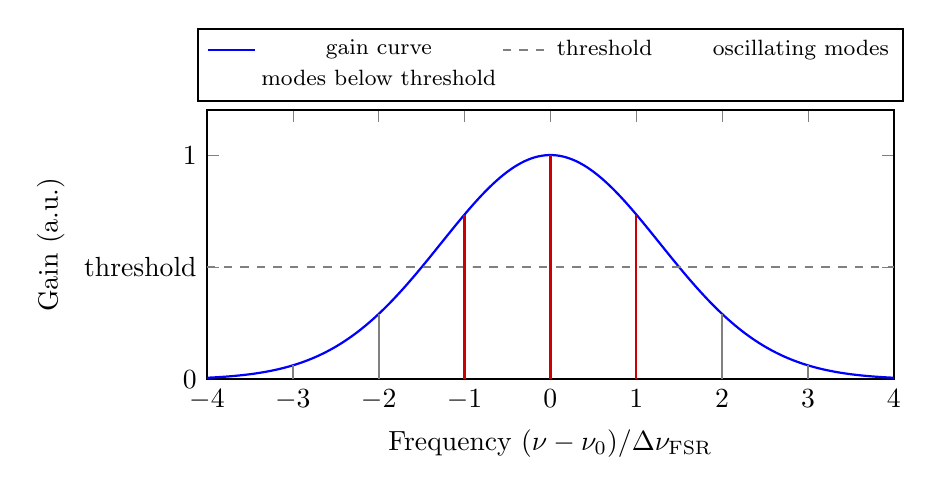
\begin{tikzpicture}
			\begin{axis}[
				width=0.85\textwidth, height=5cm,
				xlabel={Frequency $(\nu-\nu_0)/\FSR$},
				ylabel={Gain (a.u.)},
				xmin=-4, xmax=4, ymin=0, ymax=1.2,
				ytick={0,0.5,1}, yticklabels={0,threshold,1},
				samples=200, thick, no markers,
				legend style={font=\footnotesize,at={(0.5,1.03)},anchor=south,legend columns=3}]
				\addplot[blue,domain=-4:4]{exp(-x^2/3.246)};
				\addplot[dashed,gray,domain=-4:4]{0.5};
				\addplot+[ycomb,red!80!black,mark=*,thick] coordinates {(-1,0.735)(0,1)(1,0.735)};
				\addplot+[ycomb,gray,mark=o,thick] coordinates {(-3,0.0625)(-2,0.292)(2,0.292)(3,0.0625)};
				\legend{gain curve,threshold,oscillating modes,modes below threshold}
			\end{axis}
		\end{tikzpicture}
		\caption{Longitudinal modes of a cavity (spacing $\FSR=c/2nL$) under the gain curve of the medium. Only the modes whose gain exceeds the threshold oscillate; here three modes lie above threshold.}
		\label{fig:longmodes}
	\end{figure}
	
	\subsection{Transverse modes: derivation from the paraxial wave equation}
	\label{sec:transverse}
	
	The longitudinal modes tell us \emph{which frequencies} fit in the cavity. The transverse modes describe \emph{how the field is distributed across the beam}. We derive them directly from the paraxial wave equation, in five steps (Gaussian beam, then Hermite-Gaussian modes), and then use them to find the beam and the mode frequencies of a given cavity \cite{Siegman,SalehTeich,KogelnikLi1966}.
	
	\subsubsection*{Step 1: Helmholtz equation and paraxial approximation}
	
	A monochromatic wave is written $E(x,y,z,t)=\mathrm{Re}\left[U(x,y,z)\,e^{\mathrm{i}\omega t}\right]$ and its amplitude obeys the Helmholtz equation
	\begin{equation}
		\nabla^2U+k^2U=0\quad\Longrightarrow\quad
		\left(\frac{\partial^2}{\partial x^2}+\frac{\partial^2}{\partial y^2}+\frac{\partial^2}{\partial z^2}+k^2\right)U=0,
		\qquad k=\frac{n\omega}{c}=\frac{2\pi}{\lambda}.
		\label{eq:helmholtz}
	\end{equation}
	We write the field as a slowly varying complex envelope $u(x,y,z)$ multiplying a plane wave travelling along $z$:
	\begin{equation}
		U(x,y,z)=u(x,y,z)\,e^{-\mathrm{i}kz}.
	\end{equation}
	Since $\dfrac{\partial^2U}{\partial z^2}=\left(\dfrac{\partial^2u}{\partial z^2}-2\mathrm{i}k\dfrac{\partial u}{\partial z}-k^2u\right)e^{-\mathrm{i}kz}$, Eq.~\eqref{eq:helmholtz} becomes
	\begin{equation}
		\frac{\partial^2u}{\partial x^2}+\frac{\partial^2u}{\partial y^2}+\frac{\partial^2u}{\partial z^2}-2\mathrm{i}k\frac{\partial u}{\partial z}=0 .
	\end{equation}
	In the \textbf{paraxial approximation} the wave travels mostly along $z$, so the envelope changes slowly along $z$: $\left|\partial^2u/\partial z^2\right|\ll\left|k\,\partial u/\partial z\right|$. Dropping the second derivative in $z$ gives the \textbf{paraxial Helmholtz equation}
	\begin{equation}
		\frac{\partial^2u}{\partial x^2}+\frac{\partial^2u}{\partial y^2}-2\mathrm{i}k\frac{\partial u}{\partial z}=0 .
		\label{eq:paraxial}
	\end{equation}
	
	\subsubsection*{Step 2: The complex beam parameter ansatz}
	
	To solve Eq.~\eqref{eq:paraxial} we look for a beam that keeps a Gaussian profile while it spreads along $z$. We propose
	\begin{equation}
		u(x,y,z)=\psi(z)\exp\!\left[-\mathrm{i}\,\frac{k}{2q(z)}\left(x^2+y^2\right)\right],\qquad r^2=x^2+y^2,
		\label{eq:ansatz}
	\end{equation}
	where the complex \textbf{beam parameter} $q(z)$ will give both the spot size $w(z)$ and the wavefront radius $R(z)$, and $\psi(z)$ gives the amplitude and the phase on the axis. The derivatives are
	\begin{equation}
		\nabla_T^2u=\left(-\frac{2\mathrm{i}k}{q}-\frac{k^2r^2}{q^2}\right)u,\qquad
		\frac{\partial u}{\partial z}=\left(\frac{\psi'}{\psi}+\frac{\mathrm{i}k\,r^2q'}{2q^2}\right)u .
	\end{equation}
	Substituting them into Eq.~\eqref{eq:paraxial} gives
	\begin{equation}
		-\frac{2\mathrm{i}k}{q}-2\mathrm{i}k\,\frac{\psi'}{\psi}+k^2r^2\,\frac{q'-1}{q^2}=0 .
	\end{equation}
	This must hold for every $r$, so the terms in $r^2$ and the terms independent of $r$ vanish separately. We obtain two ordinary differential equations:
	\begin{equation}
		\frac{dq}{dz}=1,\qquad \frac{1}{\psi}\frac{d\psi}{dz}=-\frac{1}{q(z)} .
		\label{eq:qpsi}
	\end{equation}
	
	\subsubsection*{Step 3: Solving for $q(z)$: spot size and wavefront curvature}
	
	The first equation gives $q(z)=z+q_0$. A real $q_0$ would give a pure phase in Eq.~\eqref{eq:ansatz} (a spherical wave with no confinement), so at the waist ($z=0$) we take $q_0=\mathrm{i}z_R$ with a real length $z_R$, the Rayleigh range:
	\begin{equation}
		q(z)=z+\mathrm{i}z_R .
	\end{equation}
	(Some texts call $z_R$ by the name $z_0$.) Its inverse has a real and an imaginary part,
	\begin{equation}
		\frac{1}{q(z)}=\frac{z-\mathrm{i}z_R}{z^2+z_R^2}=\frac{z}{z^2+z_R^2}-\mathrm{i}\,\frac{z_R}{z^2+z_R^2}.
	\end{equation}
	\paragraph{How the physical parameters are obtained.} Writing the exponent of Eq.~\eqref{eq:ansatz} as $-\mathrm{i}kr^2/(2R)-r^2/w^2$ defines the wavefront radius and the spot size through
	\begin{equation}
		\frac{1}{q(z)}=\frac{1}{R(z)}-\mathrm{i}\,\frac{\lambda}{\pi w^2(z)} .
	\end{equation}
	Comparing with the previous expression:
	\begin{align}
		\frac{1}{R(z)}&=\mathrm{Re}\frac{1}{q}=\frac{z}{z^2+z_R^2}\quad\Longrightarrow\quad R(z)=z\left[1+\left(\frac{z_R}{z}\right)^2\right],\\
		\frac{\lambda}{\pi w^2(z)}&=-\mathrm{Im}\frac{1}{q}=\frac{z_R}{z^2+z_R^2}\quad\Longrightarrow\quad w^2(z)=\frac{\lambda z_R}{\pi}\left[1+\left(\frac{z}{z_R}\right)^2\right].
	\end{align}
	At $z=0$ the beam radius is the \textbf{waist} $w_0$, which fixes $z_R$. Therefore
	\begin{equation}
		\boxed{\,z_R=\frac{\pi w_0^2}{\lambda}\,},\qquad
		w(z)=w_0\sqrt{1+\left(\frac{z}{z_R}\right)^2},\qquad
		R(z)=z\left[1+\left(\frac{z_R}{z}\right)^2\right].
		\label{eq:gaussw}
	\end{equation}
	
	\subsubsection*{Step 4: Amplitude and phase on the axis, $\psi(z)$}
	
	The second equation of \eqref{eq:qpsi}, $\psi'/\psi=-1/q$, integrates to $\psi=C/q(z)$. Choosing the constant so that $\psi(0)=A_0$,
	\begin{equation}
		\psi(z)=A_0\,\frac{\mathrm{i}z_R}{z+\mathrm{i}z_R}=\frac{A_0}{1-\mathrm{i}z/z_R}=A_0\,\frac{w_0}{w(z)}\,e^{\mathrm{i}\zeta(z)},
		\qquad \zeta(z)=\arctan\frac{z}{z_R}.
		\label{eq:gaussR}
	\end{equation}
	The modulus is $\left(1+z^2/z_R^2\right)^{-1/2}=w_0/w(z)$ and the extra phase $\zeta(z)$ is the \textbf{Gouy phase}. Collecting $e^{-\mathrm{i}kz}$, the Gaussian of Eq.~\eqref{eq:ansatz} and $\psi(z)$, we obtain the fundamental Gaussian beam $\mathrm{TEM}_{00}$:
	\begin{equation}
		U_{00}(x,y,z)=A_0\,\frac{w_0}{w(z)}\exp\!\left(-\frac{x^2+y^2}{w^2(z)}\right)\exp\!\left\{-\mathrm{i}\left[kz+\frac{k\,(x^2+y^2)}{2R(z)}-\zeta(z)\right]\right\}.
		\label{eq:u00}
	\end{equation}
	The first exponential is the Gaussian amplitude profile; the second contains the plane-wave phase $kz$, the curvature of the wavefronts, and the Gouy phase. The intensity is
	\begin{equation}
		I(r,z)=I_0\left(\frac{w_0}{w(z)}\right)^{2}\exp\!\left(-\frac{2r^2}{w^2(z)}\right),\qquad I(0,z)=\frac{I_0}{1+z^2/z_R^2},
	\end{equation}
	so $w(z)$ is the radius at which the intensity falls to $1/e^2$ of its axial value (this circle contains $1-e^{-2}\approx86.5\%$ of the power), and the total power is $P=I_0\,\pi w_0^2/2$. Fig.~\ref{fig:gaussparams} shows these quantities along the axis.
	
	\begin{table}[ht]
		\centering
		\small
		\begin{tabular}{@{}p{3.3cm}p{4.6cm}p{6.2cm}@{}}
			\toprule
			Quantity & Expression & Meaning\\
			\midrule
			Rayleigh range & $z_R=\pi w_0^2/\lambda$ & distance from the waist at which the beam area doubles\\
			Beam radius at $z_R$ & $w(z_R)=\sqrt2\,w_0$ & from $w(z)$ at $z=z_R$; the beam area ($\propto w^2$) is twice the waist area, the point marked $\sqrt2\,w_0$ in Fig.~\ref{fig:gaussparams}\\
			Confocal parameter & $b=2z_R$ & depth of focus\\
			Beam radius & $w(z)=w_0\sqrt{1+(z/z_R)^2}$ & $1/e^2$ intensity radius\\
			Wavefront radius & $R(z)=z\left[1+(z_R/z)^2\right]$ & flat at the waist; minimum $2z_R$ at $z=\pm z_R$\\
			Gouy phase & $\zeta(z)=\arctan(z/z_R)$ & phase delay of $\pi$ through the focus\\
			Far-field half-angle & $\theta_{\mathrm{div}}=\lambda/(\pi w_0)$ & a small waist gives a large divergence\\
			\bottomrule
		\end{tabular}
		\caption{Parameters of the fundamental Gaussian beam, derived in Steps 3 and 4.}
		\label{tab:gauss}
	\end{table}
	
	\begin{figure}[ht]
		\centering
		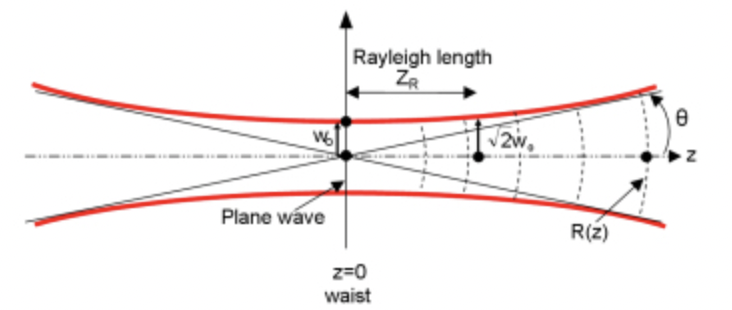
\includegraphics[width=0.85\textwidth]{images/params.png}
		\caption{Gaussian beam parameters. At the waist ($z=0$) the beam radius is $w_0$ and the wavefront is a plane wave. At $z=z_R$ (the Rayleigh length) the radius has grown to $\sqrt2\,w_0$. Farther away the wavefronts become curved with radius $R(z)$, and the beam envelope (red) approaches the asymptotes of half-angle $\theta$, the far-field divergence. Source of the figure: course \emph{Optique et Photonique Instrumentale}, Le Mans Universit\'e (F.~Varet), \url{https://perso.univ-lemans.fr/~fvaret/opi/cours_maj/OPI_ang_M01_C03_web_gen_auroraW/co/Contenu_08.html}.}
		\label{fig:gaussparams}
	\end{figure}
	
	
	\subsubsection*{Step 5: Higher-order solutions: Hermite-Gaussian modes}
	
	The Gaussian beam is the simplest solution of Eq.~\eqref{eq:paraxial}. To find the others we look for solutions in which $x$ and $y$ are separable products of a function times the fundamental beam:
	\begin{equation}
		u_{lm}(x,y,z)=X(x,z)\,Y(y,z)\,u_{00}(x,y,z),
	\end{equation}
	where $u_{00}$ is the envelope of Step~4 (Eq.~\eqref{eq:u00} without the factor $e^{-\mathrm{i}kz}$). Inserting this in Eq.~\eqref{eq:paraxial}, the terms that contain only $u_{00}$ cancel because $u_{00}$ is already a solution. Using $\partial_xu_{00}/u_{00}=-\mathrm{i}kx/q$, what remains for the $x$-dependent factor is
	\begin{equation}
		\frac{\partial^2X}{\partial x^2}-\frac{2\mathrm{i}k\,x}{q}\frac{\partial X}{\partial x}-2\mathrm{i}k\,\frac{\partial X}{\partial z}=0 ,
	\end{equation}
	and the same equation holds for $Y(y,z)$. We try
	\begin{equation}
		X(x,z)=H_l(\xi)\,e^{\mathrm{i}l\zeta(z)},\qquad \xi=\frac{\sqrt2\,x}{w(z)} ,
	\end{equation}
	where the phase factor $e^{\mathrm{i}l\zeta}$ is needed to make the equation separate. The following relations, which follow from Steps 3 and 4, are used in the substitution:
	\begin{equation}
		\frac{w'}{w}=\frac{z}{z^2+z_R^2},\quad
		\zeta'=\frac{z_R}{z^2+z_R^2},\quad
		\frac1q=\frac{z-\mathrm{i}z_R}{z^2+z_R^2},\quad
		\frac{2}{w^2}=\frac{k\,z_R}{z^2+z_R^2}.
	\end{equation}
	With $\partial_x=(\sqrt2/w)\,\partial_\xi$ and $\partial_z\xi=-\xi\,w'/w$, the equation for $X$ becomes
	\begin{equation}
		\frac{k\,z_R}{z^2+z_R^2}\left[\frac{d^2H_l}{d\xi^2}-2\xi\frac{dH_l}{d\xi}+2l\,H_l\right]=0 ,
	\end{equation}
	which is \textbf{Hermite's differential equation}. Solutions that remain finite for large $\xi$ exist only for integer $l=0,1,2,\dots$, and they are the Hermite polynomials
	\begin{equation}
		H_0=1,\qquad H_1(\xi)=2\xi,\qquad H_2(\xi)=4\xi^2-2,\qquad H_3(\xi)=8\xi^3-12\xi,\ \dots
	\end{equation}
	The same holds for $y$ with an integer $m$. Each unit of $l$ or $m$ adds one more factor $e^{\mathrm{i}\zeta}$, so the Gouy phase becomes $(l+m+1)\,\zeta(z)$. Putting the polynomials together with the Gaussian envelope gives the complete \textbf{Hermite-Gaussian mode} $\mathrm{TEM}_{lm}$:
	\begin{equation}
		U_{lm}(x,y,z)=A_{lm}\,\frac{w_0}{w(z)}\,H_l\!\left[\frac{\sqrt2\,x}{w(z)}\right]H_m\!\left[\frac{\sqrt2\,y}{w(z)}\right]
		e^{-\frac{x^2+y^2}{w^2(z)}}\,
		\exp\!\left\{-\mathrm{i}\left[kz+\frac{k\,(x^2+y^2)}{2R(z)}-(l+m+1)\,\zeta(z)\right]\right\}.
		\label{eq:hg}
	\end{equation}
	Compared with the fundamental mode, $w(z)$ and $R(z)$ are the same, so \emph{all} modes of a cavity fit the same mirrors. What changes is the pattern: $l$ and $m$ count the nodal lines along $x$ and $y$, the pattern grows with the order (its extent is approximately proportional to $\sqrt{l+m+1}\,w$), and the Gouy phase accumulates $l+m+1$ times faster (Figs.~\ref{fig:hgmodes} and \ref{fig:hgsurf}). In cavities with circular symmetry the same family is written with Laguerre-Gaussian modes $\mathrm{TEM}_{p\ell}$, for which $l+m$ is replaced by $2p+|\ell|$.
	
	\begin{figure}[ht]
		\centering
		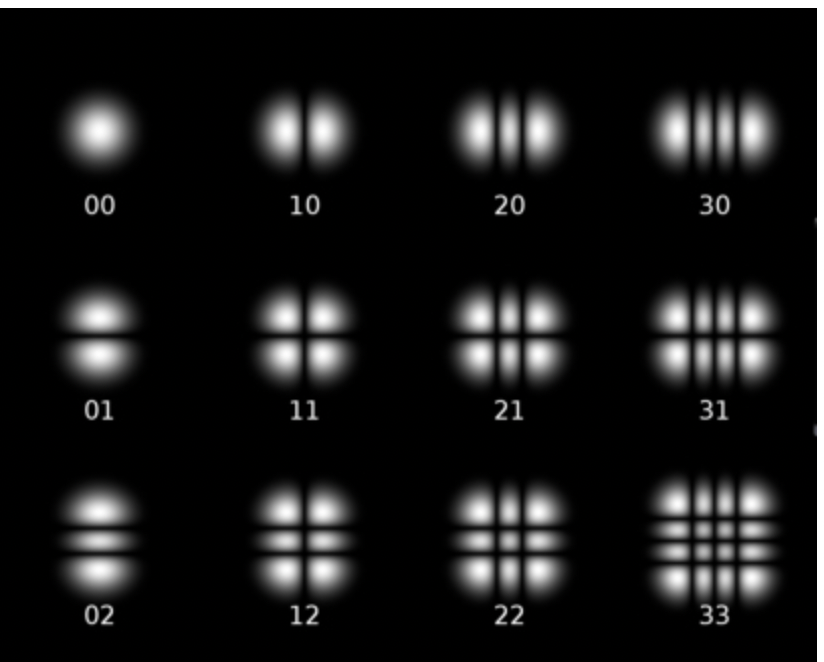
\includegraphics[width=0.78\textwidth]{images/modes.png}
		\caption{Transverse intensity patterns $|U_{lm}|^2$ of Hermite-Gaussian modes $\mathrm{TEM}_{lm}$ (the labels give $lm$). The first index $l$ counts the dark nodal lines along $x$ and the second index $m$ along $y$, so $\mathrm{TEM}_{00}$ is a single spot, $\mathrm{TEM}_{10}$ has two lobes side by side, and $\mathrm{TEM}_{33}$ has a $4\times4$ array of lobes. The pattern grows with the order, as stated after Eq.~\eqref{eq:hg}. Source: Le Mans Universit\'e course (F.~Varet), \url{https://perso.univ-lemans.fr/~fvaret/opi/cours_maj/OPI_ang_M01_C03_web_gen_auroraW/co/Contenu_13.html}.}
		\label{fig:hgmodes}
	\end{figure}
	
	\begin{figure}[ht]
		\centering
		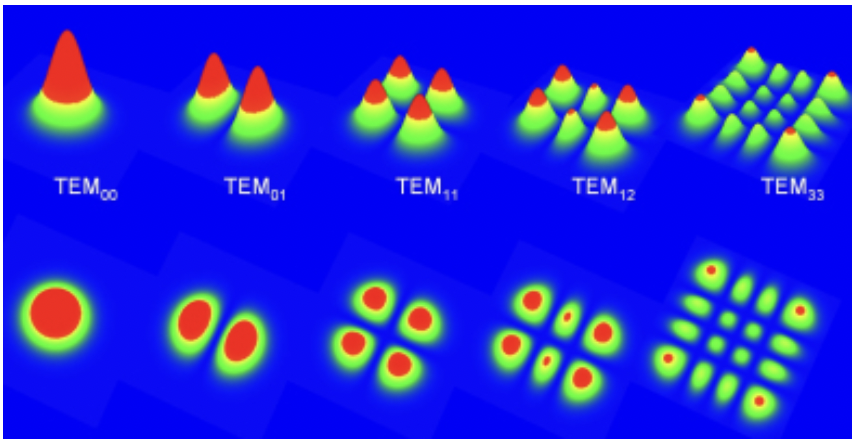
\includegraphics[width=0.85\textwidth]{images/modes_jet.png}
		\caption{The same family seen as intensity surfaces (top) and as 2D maps (bottom) for $\mathrm{TEM}_{00}$, $\mathrm{TEM}_{01}$, $\mathrm{TEM}_{11}$, $\mathrm{TEM}_{12}$ and $\mathrm{TEM}_{33}$. Every bright lobe is a peak of the intensity and the lobes are separated by nodal lines where the field changes sign. Source: Le Mans Universit\'e course (F.~Varet), see the link in Fig.~\ref{fig:hgmodes}.}
		\label{fig:hgsurf}
	\end{figure}
	
	
	\subsubsection*{Step 6: Fitting the beam to the cavity}
	
	The cavity selects the beam whose wavefronts coincide with the mirror surfaces, so that the beam retraces itself after reflection. Place the waist at $z=0$ and the mirrors at $z_1<0$ and $z_2>0$, so that $L=z_2-z_1$. With radii $R_{c1},R_{c2}>0$ for concave mirrors, the matching conditions are $R(z_1)=-R_{c1}$ and $R(z_2)=+R_{c2}$, that is, with $R(z)=z+z_R^2/z$,
	\begin{equation}
		z_2+\frac{z_R^2}{z_2}=R_{c2},\qquad z_1+\frac{z_R^2}{z_1}=-R_{c1},\qquad z_2-z_1=L .
	\end{equation}
	These are three equations for the three unknowns $z_1$, $z_2$ and $z_R$. Solving them gives
	\begin{equation}
		z_R^2=\frac{L\,(R_{c1}-L)(R_{c2}-L)(R_{c1}+R_{c2}-L)}{(R_{c1}+R_{c2}-2L)^2},\quad
		z_1=-\frac{L\,(R_{c2}-L)}{R_{c1}+R_{c2}-2L},\quad
		z_2=\frac{L\,(R_{c1}-L)}{R_{c1}+R_{c2}-2L}.
		\label{eq:cavmatch}
	\end{equation}
	In terms of $g_i=1-L/R_{ci}$ (Eq.~\eqref{eq:gparam}), $z_R^2=L^2g_1g_2(1-g_1g_2)/(g_1+g_2-2g_1g_2)^2$, which has a real solution only for $0<g_1g_2<1$, the stability condition of Sec.~\ref{sec:stability}. Checks: for a symmetric cavity $z_R^2=L(2R_c-L)/4$; for a plano-concave cavity ($R_{c1}\to\infty$) $z_1=0$, so the waist lies on the flat mirror, and $z_R^2=L(R_{c2}-L)$; for the confocal cavity $z_R=L/2$.
	
	\textbf{Procedure.} To find the beam in a given cavity: (i) compute $g_1,g_2$ and check $0<g_1g_2<1$; (ii) compute $z_R$, $z_1$, $z_2$ from Eq.~\eqref{eq:cavmatch}; (iii) the waist is $w_0=\sqrt{\lambda z_R/\pi}$; (iv) the spot sizes on the mirrors are $w_i=w_0\sqrt{1+z_i^2/z_R^2}$; (v) the far-field divergence is $\lambda/\pi w_0$; (vi) the mode frequencies follow from Step~7. A numerical example is worked out in Sec.~\ref{sec:examples}.
	
	\subsubsection*{Step 7: Resonance frequencies of the transverse modes}
	
	From Eq.~\eqref{eq:hg} the on-axis phase of the mode $\mathrm{TEM}_{lm}$ is $\phi(0,0,z)=kz-(l+m+1)\,\zeta(z)$. After one round trip between the mirrors at $z_1$ and $z_2$, the accumulated phase is
	\begin{align}
		\text{round-trip phase}&=2\left[\phi(0,0,z_2)-\phi(0,0,z_1)\right]\nonumber\\
		&=2\left[kz_2-(l+m+1)\zeta(z_2)-kz_1+(l+m+1)\zeta(z_1)\right]\nonumber\\
		&=2kL-2(l+m+1)\,\Delta\zeta,\qquad \Delta\zeta=\zeta(z_2)-\zeta(z_1).
	\end{align}
	The field reproduces itself only if this phase is an integer multiple of $2\pi$:
	\begin{equation}
		q\cdot2\pi=2kL-2(l+m+1)\,\Delta\zeta .
	\end{equation}
	With $k=2\pi\nu n/c$, this becomes
	\begin{equation}
		q\cdot2\pi=2\cdot\frac{2\pi\nu_q}{c}\,nL-2(l+m+1)\,\Delta\zeta
		\;\Longrightarrow\;
		\boxed{\,\nu_q=q\,\frac{c}{2nL}+\frac{\Delta\zeta}{\pi}\,(l+m+1)\,\frac{c}{2nL}\,}
		\label{eq:transfreq}
	\end{equation}
	or, with $\nu_F=c/2nL$ the free spectral range, $\nu_q=q\,\nu_F+\dfrac{\Delta\zeta}{\pi}(l+m+1)\,\nu_F$. The first term is the longitudinal comb of Eq.~\eqref{eq:longmodes}. The second term shifts each transverse mode by a fraction of the FSR. The FSR is therefore the same as for the passive Fabry-P\'erot interferometer, and the transverse indices only add an offset.
	
	\paragraph{The Gouy-phase shift in terms of the mirrors.} From $z=z_R\tan\zeta$,
	\begin{equation}
		\tan\Delta\zeta=\frac{\tan\zeta_2-\tan\zeta_1}{1+\tan\zeta_1\tan\zeta_2}=\frac{L\,z_R}{z_R^2+z_1z_2}.
	\end{equation}
	Using Eq.~\eqref{eq:cavmatch}, $z_R^2+z_1z_2=L(R_{c1}-L)(R_{c2}-L)/(R_{c1}+R_{c2}-2L)$, so
	\begin{equation}
		\tan^2\Delta\zeta=\frac{L\,(R_{c1}+R_{c2}-L)}{(R_{c1}-L)(R_{c2}-L)},\qquad
		1+\tan^2\Delta\zeta=\frac{R_{c1}R_{c2}}{(R_{c1}-L)(R_{c2}-L)} .
	\end{equation}
	Therefore $\cos^2\Delta\zeta=(1-L/R_{c1})(1-L/R_{c2})=g_1g_2$, and
	\begin{equation}
		\Delta\zeta=\arccos\!\left(\pm\sqrt{g_1g_2}\right),
		\label{eq:dzeta}
	\end{equation}
	with the sign $+$ when $g_1,g_2>0$ and $-$ when both are negative \cite{KogelnikLi1966,Siegman}.
	
	\begin{table}[ht]
		\centering
		\small
		\begin{tabular}{@{}p{3.6cm}cccp{4.6cm}@{}}
			\toprule
			Cavity & $g_1g_2$ & $\Delta\zeta/\pi$ & Offset per order & Consequence\\
			\midrule
			Plane-plane & $1$ & $0$ & none & all $\mathrm{TEM}_{lm}$ degenerate\\
			Plano-concave, $L=0.3$\,m, $R_{c2}=0.5$\,m & $0.4$ & $0.282$ & $0.282\,\nu_F$ & $\Delta\nu_T\approx141$\,MHz\\
			Symmetric confocal & $0$ & $1/2$ & $\nu_F/2$ & even and odd orders interleave, spacing $c/4L$\\
			Concentric & $1$ (both $g<0$) & $1$ & $\nu_F$ & all $\mathrm{TEM}_{lm}$ degenerate\\
			\bottomrule
		\end{tabular}
		\caption{Transverse mode offsets for typical cavities, from Eqs.~\eqref{eq:transfreq} and \eqref{eq:dzeta}.}
		\label{tab:dzeta}
	\end{table}
	
	Three conclusions follow:
	\begin{itemize}
		\item Modes with the same $q$ and different order $N=l+m$ are separated by $\Delta\nu_T=\dfrac{\Delta\zeta}{\pi}\,\nu_F$ per unit of $N$, a fraction of the longitudinal spacing.
		\item All modes with the same $N=l+m$ have the same frequency (they are degenerate), and there are $N+1$ of them. The degeneracy is lifted by asymmetries such as astigmatic mirrors or an aperture.
		\item In the plane-plane and concentric limits $\Delta\zeta/\pi=0$ or $1$, so all transverse modes of a given $q$ coincide. In the confocal cavity $\Delta\zeta/\pi=1/2$: modes of even $N$ coincide with the longitudinal comb and modes of odd $N$ fall exactly half-way between, which gives the spectrum with spacing $c/4L$ used in the confocal scanning interferometer (Sec.~\ref{sec:examples}).
	\end{itemize}
	
	
	\subsubsection*{Which transverse mode oscillates?}
	
	The mirrors and the Gaussian beam fit all the modes, but not all of them oscillate. Higher-order modes are wider than $\mathrm{TEM}_{00}$ and therefore suffer more loss at any aperture (the gain tube, a mirror edge, or an intracavity iris). A laser usually runs on the $\mathrm{TEM}_{00}$ mode because it has the smallest size, the lowest diffraction loss and the best beam quality. Higher-order modes are suppressed with an intracavity aperture, or by choosing a cavity geometry whose fundamental mode is the only one with sufficient overlap with the gain region. Conversely, a large pumped volume and a large mode size allow several $(l,m)$ modes to oscillate together and give a multimode beam.
	
	
	
	
	%==========================================================================
	\section{Cavity Configuration and Stability}
	\label{sec:stability}
	%==========================================================================
	
	\subsection{Ray-matrix derivation}
	
	Not every pair of mirrors can trap light. If the mirrors are curved the wrong way, a ray that is slightly off-axis walks away after a few round trips. The geometric condition for stable confinement follows from ray-transfer (ABCD) matrices \cite{KogelnikLi1966,Siegman,SalehTeich}. Let the mirror radii $R_{c1}$, $R_{c2}$ be positive for concave mirrors (centre of curvature inside the cavity). For one round trip, the matrix is the product of free propagation over $L$ and reflection from a mirror of radius $R_c$ (a focusing element with $f=R_c/2$):
	\begin{equation}
		M=\begin{pmatrix}1&0\\-2/R_{c2}&1\end{pmatrix}
		\begin{pmatrix}1&L\\0&1\end{pmatrix}
		\begin{pmatrix}1&0\\-2/R_{c1}&1\end{pmatrix}
		\begin{pmatrix}1&L\\0&1\end{pmatrix}.
	\end{equation}
	Since $\det M=1$, the ray after $N$ round trips remains bounded only if $|A+D|/2\le 1$, where $A$ and $D$ are the diagonal elements of $M$. Defining the \textbf{cavity $g$-parameters}
	\begin{equation}
		g_1=1-\frac{L}{R_{c1}},\qquad g_2=1-\frac{L}{R_{c2}},
		\label{eq:gparam}
	\end{equation}
	one finds $(A+D)/2=2g_1g_2-1$. The stability condition $-1\le 2g_1g_2-1\le 1$ is then
	\begin{equation}
		\boxed{\,0\le g_1g_2\le 1\,}
		\label{eq:stability}
	\end{equation}
	The same result is obtained from the Gaussian-beam picture: a Gaussian beam of the form \eqref{eq:gaussw}--\eqref{eq:gaussR} fits the cavity only when its wavefronts coincide with the mirror surfaces, $R(z_i)=R_{ci}$, and this has a real solution only when \eqref{eq:stability} holds \cite{KogelnikLi1966}.
	
	\subsection{The stability diagram}
	
	The condition \eqref{eq:stability} is displayed in the $(g_1,g_2)$ plane in Fig.~\ref{fig:stabdiag}. The stable region lies between the axes and the hyperbola $g_1g_2=1$, in the first and third quadrants. Common cavities are points in this diagram. A cavity is \emph{unstable} when $g_1g_2<0$ or $g_1g_2>1$. Cavities exactly on the boundary are \emph{marginally stable}, and a tiny change of mirror spacing or tilt decides whether they work.
	
	\begin{figure}[ht]
		\centering
		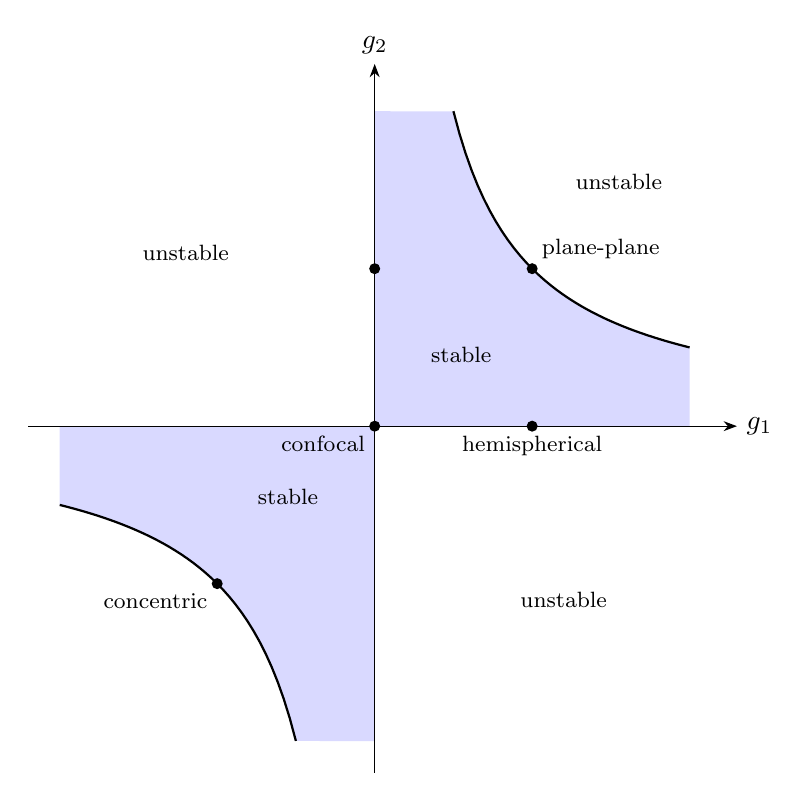
\begin{tikzpicture}[scale=2.0,>=Stealth]
			\fill[blue!15] (0,0)--(2,0)--(2,0.5)--plot[domain=2:0.5,samples=40]({\x},{1/\x})--(0,2)--cycle;
			\fill[blue!15] (0,0)--(-2,0)--(-2,-0.5)--plot[domain=-2:-0.5,samples=40]({\x},{1/\x})--(0,-2)--cycle;
			\draw[->] (-2.2,0) -- (2.3,0) node[right] {$g_1$};
			\draw[->] (0,-2.2) -- (0,2.3) node[above] {$g_2$};
			\draw[thick,domain=0.5:2,samples=40] plot ({\x},{1/\x});
			\draw[thick,domain=-2:-0.5,samples=40] plot ({\x},{1/\x});
			% points
			\fill (1,1) circle (0.035) node[above right,font=\footnotesize] {plane-plane};
			\fill (0,0) circle (0.035) node[below left,font=\footnotesize] {confocal};
			\fill (-1,-1) circle (0.035) node[below left,font=\footnotesize] {concentric};
			\fill (1,0) circle (0.035) node[below,font=\footnotesize] {hemispherical};
			\fill (0,1) circle (0.035);
			\node[font=\footnotesize] at (0.55,0.45) {stable};
			\node[font=\footnotesize] at (-0.55,-0.45) {stable};
			\node[font=\footnotesize] at (-1.2,1.1) {unstable};
			\node[font=\footnotesize] at (1.2,-1.1) {unstable};
			\node[font=\footnotesize] at (1.55,1.55) {unstable};
		\end{tikzpicture}
		\caption{Stability diagram of a two-mirror resonator: the shaded areas satisfy $0\le g_1g_2\le1$ and the curves are $g_1g_2=1$. The named points are the standard special configurations.}
		\label{fig:stabdiag}
	\end{figure}
	
	\begin{table}[ht]
		\centering
		\small
		\begin{tabular}{@{}lccccl@{}}
			\toprule
			Configuration & $R_{c1}$ & $R_{c2}$ & $g_1$ & $g_2$ & Status\\
			\midrule
			Plane-plane (flat \FP{}) & $\infty$ & $\infty$ & $1$ & $1$ & marginal\\
			Symmetric confocal & $L$ & $L$ & $0$ & $0$ & stable (boundary)\\
			Concentric (spherical) & $L/2$ & $L/2$ & $-1$ & $-1$ & marginal\\
			Hemispherical & $\infty$ & $L$ & $1$ & $0$ & stable (boundary)\\
			Plano-concave & $\infty$ & $R_{c2}>L$ & $1$ & $0<g_2<1$ & stable\\
			Symmetric, $R_c>L$ (long radius) & $R_c$ & $R_c$ & $g$ & $g$ & stable\\
			Convex-concave / $R_c<L/2$ (e.g.) & --- & --- & $g_1g_2<0$ or $>1$ & & unstable\\
			\bottomrule
		\end{tabular}
		\caption{Common two-mirror cavity configurations and their stability.}
		\label{tab:configs}
	\end{table}
	
	\subsection{Beam parameters of a stable cavity}
	
	For a stable cavity, solving $R(z_i)=R_{ci}$ gives the position of the waist and the spot sizes in terms of $g_1$, $g_2$ and $L$ \cite{KogelnikLi1966,Siegman,Svelto}. The waist is located a distance $z_1$ from mirror~1,
	\begin{equation}
		z_1=\frac{L\,g_2(1-g_1)}{g_1+g_2-2g_1g_2},
	\end{equation}
	and the waist radius and the spot sizes on the mirrors are
	\begin{align}
		w_0^2 &= \frac{\lambda L}{\pi}\,\frac{\sqrt{g_1g_2(1-g_1g_2)}}{\left|g_1+g_2-2g_1g_2\right|},\\
		w_1^2 &= \frac{\lambda L}{\pi}\sqrt{\frac{g_2}{g_1(1-g_1g_2)}}, \qquad
		w_2^2 = \frac{\lambda L}{\pi}\sqrt{\frac{g_1}{g_2(1-g_1g_2)}}.
		\label{eq:spots}
	\end{align}
	For a symmetric cavity ($g_1=g_2=g$), the waist lies at the centre, $z_1=L/2$, with
	\begin{equation}
		w_0^2=\frac{\lambda L}{2\pi}\sqrt{\frac{1+g}{1-g}},\qquad w_1^2=w_2^2=\frac{\lambda L}{\pi}\frac{1}{\sqrt{1-g^2}} .
		\label{eq:symm}
	\end{equation}
	For a plano-concave cavity ($R_{c1}=\infty$, $g_1=1$) the waist lies on the flat mirror and $w_0^2=(\lambda/\pi)\sqrt{L(R_{c2}-L)}$, with Rayleigh range $z_R=\sqrt{L(R_{c2}-L)}$. All spot sizes diverge as $g_1g_2\to1$, which marks the edge of stability.
	
	%==========================================================================
	\section{Influence of Cavity Stability on Laser Performance}
	%==========================================================================
	
	The position of the cavity in the $(g_1,g_2)$ diagram determines how the laser behaves in practice. The main effects are:
	
	\textbf{Mode size and gain extraction.} The mode volume of the $\mathrm{TEM}_{00}$ beam must overlap the pumped region of the gain medium. A large fundamental mode (cavities near the plane-plane or concentric points) fills a large volume of active material and can extract more power, but it also tends to let several transverse modes oscillate. A small mode (confocal and near-confocal) concentrates the field, giving a higher intensity for a given power and a lower threshold in small gain volumes, but it samples less of the medium. In end-pumped solid-state lasers, the pump spot and the cavity waist are therefore chosen together (mode matching).
	
	\begin{figure}[ht]
		\centering
		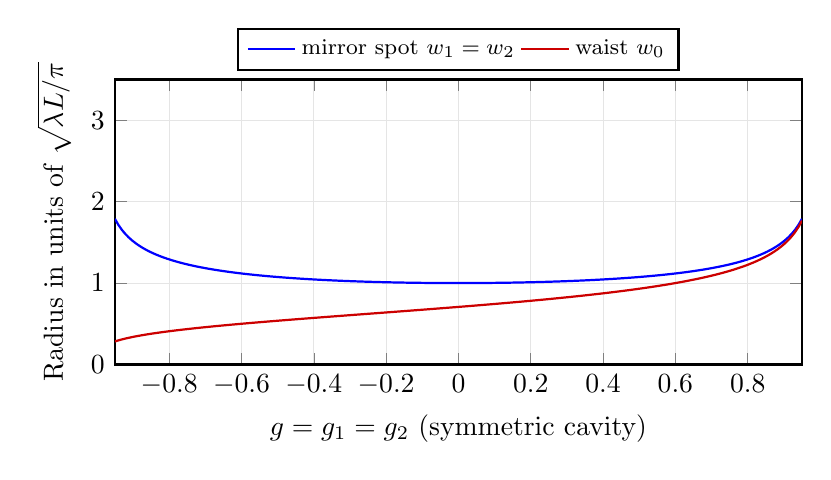
\begin{tikzpicture}
			\begin{axis}[
				width=0.85\textwidth, height=5.2cm,
				xlabel={$g=g_1=g_2$ (symmetric cavity)},
				ylabel={Radius in units of $\sqrt{\lambda L/\pi}$},
				xmin=-0.95, xmax=0.95, ymin=0, ymax=3.5,
				samples=200, thick, no markers, grid=both, grid style={gray!20},
				legend style={font=\footnotesize,at={(0.5,1.03)},anchor=south,legend columns=2}]
				\addplot[blue,domain=-0.95:0.95]{(1-x^2)^(-0.25)};
				\addplot[red!80!black,domain=-0.95:0.95]{((1+x)/(1-x))^0.25/sqrt(2)};
				\legend{mirror spot $w_1=w_2$, waist $w_0$}
			\end{axis}
		\end{tikzpicture}
		\caption{Spot sizes of a symmetric cavity, from Eq.~\eqref{eq:symm}. Near $g=\pm1$ (plane-plane and concentric limits) the mirror spot grows without bound; at $g=0$ (confocal) the beam is smallest on the mirrors. The waist is largest as $g\to1$ and vanishes as $g\to-1$.}
		\label{fig:spotsizes}
	\end{figure}
	
	\textbf{Misalignment sensitivity.} Near the stability boundaries, $1-g_1g_2\to 0$ or $g_1g_2\to0$ in a way that makes the mode size diverge or collapse (Fig.~\ref{fig:spotsizes}). Here a tiny tilt of one mirror moves the axis of the mode a long way across the mirrors, and the beam may walk off the aperture or the gain region, so the output power drops quickly. Plane-plane and concentric cavities are the most delicate. A cavity placed near the middle of the stable region (such as $g_1g_2\approx0.3$--$0.7$) tolerates mirror tilt and spacing drift much better, which is why it is the default choice for commercial lasers \cite{Siegman,HodgsonWeber}.
	
	\textbf{Transverse mode content and beam quality.} Large fundamental modes (small $|{\arccos\sqrt{g_1g_2}}|$) have closely spaced and nearly degenerate transverse modes, and diffraction losses differ little between the $\mathrm{TEM}_{00}$ mode and higher orders. The laser tends to oscillate on several transverse modes, which degrades the beam quality factor $M^2$. Fox and Li characterised this with the \emph{Fresnel number} $N_F=a^2/(\lambda L)$, where $a$ is the mirror (or aperture) radius: high-order modes suffer much larger diffraction loss when $N_F$ is small, which is why a limiting aperture is an effective mode filter \cite{FoxLi1961}.
	
	\textbf{Output divergence.} The far-field half-angle of the output is $\theta_{\mathrm{div}}=\lambda/(\pi w_0)$. A small waist therefore gives a strongly divergent beam, and a large one a well-collimated beam. A cavity with a long Rayleigh range (large $w_0$) is attractive for applications requiring a collimated output.
	
	\textbf{Thermal effects.} Pumping a solid-state gain medium heats it and creates a thermal lens, which changes the effective $g$-parameters. A cavity operated near a stability edge may switch from stable to unstable when the pump power rises, so output power and mode shape change abruptly. Resonators are therefore designed to be stable over the whole range of thermal-lens focal lengths \cite{Svelto}.
	
	\textbf{Unstable resonators.} In high-gain, high-power lasers the stable cavity has too small a mode volume to extract all the energy. An \emph{unstable} cavity ($g_1g_2<0$ or $>1$) lets the beam expand until it fills the whole gain volume, and the output is coupled out around the edge of a mirror. It has a high gain extraction but a different output profile \cite{Siegman}.
	
	%==========================================================================
	\section{Practical Example and Applications}
	\label{sec:examples}
	%==========================================================================
	
	\subsection{Worked example: a helium-neon laser}
	
	A small helium-neon laser at $\lambda=\SI{632.8}{nm}$ typically has a cavity length of about $L=\SI{0.30}{m}$ with a flat high reflector and a concave output coupler. We take the plano-concave case $R_{c1}=\infty$, $R_{c2}=\SI{0.50}{m}$, which gives
	\begin{equation}
		g_1=1,\qquad g_2=1-\frac{0.30}{0.50}=0.40,\qquad g_1g_2=0.40.
	\end{equation}
	Since $0<g_1g_2<1$, the cavity is stable and lies comfortably inside the stable region. The Gaussian beam follows from Eq.~\eqref{eq:spots}:
	\begin{align*}
		w_0 &= \sqrt{\frac{\lambda}{\pi}\sqrt{L(R_{c2}-L)}}=\sqrt{2.01\times10^{-7}\,\mathrm{m}\times0.245\,\mathrm{m}}\approx\SI{0.22}{mm}\quad(\text{on the flat mirror}),\\
		z_R &= \sqrt{L(R_{c2}-L)}\approx\SI{0.245}{m},\\
		w_2 &= \sqrt{\frac{\lambda L}{\pi}\sqrt{\frac{g_1}{g_2(1-g_1g_2)}}}\approx\SI{0.35}{mm}\quad(\text{on the output coupler}),
	\end{align*}
	and a far-field half-angle $\theta_{\mathrm{div}}=\lambda/(\pi w_0)\approx\SI{0.9}{mrad}$. The longitudinal mode spacing is
	\begin{equation}
		\FSR=\frac{c}{2L}=\frac{2.998\times10^{8}}{0.60}\approx\SI{500}{MHz},
	\end{equation}
	and the neon gain is Doppler-broadened to a width of about $\SI{1.5}{GHz}$, so about three longitudinal modes can lie above threshold (compare Fig.~\ref{fig:longmodes}). The transverse mode spacing is, from Eq.~\eqref{eq:transfreq},
	\begin{equation}
		\Delta\nu_T=\FSR\,\frac{\arccos\sqrt{0.40}}{\pi}\approx 500\ \mathrm{MHz}\times0.282\approx\SI{141}{MHz}.
	\end{equation}
	Because the aperture of the narrow discharge tube introduces large diffraction losses for the higher-order modes, the laser runs on the $\mathrm{TEM}_{00}$ mode and yields a clean Gaussian beam. If the mirror $M_2$ were replaced by one with $R_{c2}=\SI{0.30}{m}$ (the hemispherical limit, $g_2=0$), the cavity would sit on the stability boundary and the laser would become sensitive to tiny misalignments, which illustrates the importance of Sec.~\ref{sec:stability}.
	
	\subsection{Semiconductor laser diode}
	
	The edge-emitting laser diode is a \FP{} cavity in which the mirrors are simply the cleaved facets of the crystal. For a semiconductor of refractive index $n\approx3.5$ the facet reflectivity is $R=\left(\frac{n-1}{n+1}\right)^2\approx0.31$, which is high enough because the gain is large. For a cavity length $L=\SI{300}{\micro m}$, the mirror-loss term of Eq.~\eqref{eq:threshold} is $(1/L)\ln(1/R)\approx\SI{39}{cm^{-1}}$. With a group index $n_g\approx4$ the mode spacing is $c/(2n_gL)\approx\SI{125}{GHz}$, that is, $\Delta\lambda\approx\SI{0.3}{nm}$ at $\SI{850}{nm}$, so the spectrum of a multimode \FP{} diode laser is a comb of lines about $\SI{0.3}{nm}$ apart under the gain bandwidth \cite{Coldren}. Here the transverse modes are determined by the semiconductor waveguide rather than by curved mirrors, so the stability analysis above does not apply.
	
	\subsection{The confocal scanning interferometer}
	
	A spherical-mirror \FP{} interferometer with $R_{c1}=R_{c2}=L$ (confocal) is the standard instrument for observing the longitudinal modes of lasers. In this geometry a ray retraces its path after \emph{two} round trips, so the free spectral range is $c/4L$, and all modes of the cavity are transmitted at the same frequencies, which makes the instrument insensitive to the exact alignment and to the transverse profile of the laser beam, in contrast with the plane-plane etalon. A piezo scans $L$ by a fraction of a wavelength and a photodiode shows the mode comb of the laser under test, such as the three modes of the HeNe laser above \cite{Hernandez,Vaughan}.
	
	\subsection{Other applications}
	
	\begin{itemize}
		\item \textbf{Optical filters and telecommunications.} Thin etalons act as narrow-band filters in wavelength-division multiplexing and as wavelength references for laser frequency locking \cite{Hecht,Yariv}.
		\item \textbf{Laser frequency stabilisation.} A high-finesse cavity serves as a frequency discriminator. In the Pound-Drever-Hall technique the laser is locked to a cavity resonance, which narrows its linewidth far below the cavity linewidth \cite{Drever1983}.
		\item \textbf{Gravitational-wave detection.} The kilometre-scale arms of LIGO are \FP{} cavities with a finesse of several hundred, which multiplies the effective path length and thus the phase signal of a passing gravitational wave \cite{Abbott2009}.
		\item \textbf{Cavity-enhanced spectroscopy and sensing.} The long effective path in a high-finesse cavity makes weak absorptions measurable, and the resonance shifts when the optical path changes, so cavities also work as sensors of length, refractive index, temperature and pressure.
	\end{itemize}
	
	%==========================================================================
	\section{Conclusion}
	%==========================================================================
	
	The \FP{} structure combines two simple ideas, multiple-beam interference and optical feedback, into a device with several different uses. As an interferometer, its transmission is given by the Airy function, with a free spectral range $c/2nd$ and a finesse $\pi\sqrt R/(1-R)$ that together define its resolving power. As a laser resonator, the same geometry fixes the longitudinal mode spacing $c/2nL$ and, through the curvature of the mirrors, the transverse modes of the Gaussian beam. Stability requires $0\le g_1g_2\le1$, and the position inside this region determines the mode size, the number of transverse modes, the tolerance to misalignment and the robustness against thermal effects. Practical designs therefore avoid the boundaries of the stability diagram unless a particular property, such as a large mode volume or a very small waist, is needed.
	
	%==========================================================================
	\begin{thebibliography}{99}
		\bibitem{FabryPerot1899} C.~Fabry and A.~Perot, ``On the Application of Interference Phenomena to the Solution of Various Problems of Spectroscopy and Metrology'' \emph{The Astrophysical Journal} \textbf{9}, 87--115 (1899).
		\bibitem{BornWolf} M.~Born and E.~Wolf, \emph{Principles of Optics}, 7th ed. (Cambridge University Press, Cambridge, 1999), Chap.~7.
		\bibitem{Hecht} E.~Hecht, \emph{Optics}, 5th ed. (Pearson, Boston, 2017).
		\bibitem{SalehTeich} B.~E.~A. Saleh and M.~C. Teich, \emph{Fundamentals of Photonics}, 3rd ed. (Wiley, Hoboken, 2019).
		\bibitem{Siegman} A.~E. Siegman, \emph{Lasers} (University Science Books, Mill Valley, 1986).
		\bibitem{Svelto} O.~Svelto, \emph{Principles of Lasers}, 5th ed. (Springer, New York, 2010).
		\bibitem{Milonni} P.~W. Milonni and J.~H. Eberly, \emph{Laser Physics} (Wiley, Hoboken, 2010).
		\bibitem{Yariv} A.~Yariv and P.~Yeh, \emph{Photonics: Optical Electronics in Modern Communications}, 6th ed. (Oxford University Press, New York, 2007).
		\bibitem{Vaughan} J.~M. Vaughan, \emph{The Fabry-Perot Interferometer: History, Theory, Practice and Applications} (Adam Hilger, Bristol, 1989).
		\bibitem{Hernandez} G.~Hernandez, \emph{Fabry-Perot Interferometers} (Cambridge University Press, Cambridge, 1986).
		\bibitem{HodgsonWeber} N.~Hodgson and H.~Weber, \emph{Laser Resonators and Beam Propagation}, 2nd ed. (Springer, New York, 2005).
		\bibitem{Coldren} L.~A. Coldren, S.~W. Corzine, and M.~L. Ma\v{s}anovi\'c, \emph{Diode Lasers and Photonic Integrated Circuits}, 2nd ed. (Wiley, Hoboken, 2012).
		\bibitem{SchawlowTownes1958} A.~L. Schawlow and C.~H. Townes, ``Infrared and optical masers,'' \emph{Phys. Rev.} \textbf{112}, 1940--1949 (1958).
		\bibitem{Maiman1960} T.~H. Maiman, ``Stimulated optical radiation in ruby,'' \emph{Nature} \textbf{187}, 493--494 (1960).
		\bibitem{FoxLi1961} A.~G. Fox and T.~Li, ``Resonant modes in a maser interferometer,'' \emph{Bell Syst. Tech. J.} \textbf{40}, 453--488 (1961).
		\bibitem{KogelnikLi1966} H.~Kogelnik and T.~Li, ``Laser beams and resonators,'' \emph{Appl. Opt.} \textbf{5}, 1550--1567 (1966).
		\bibitem{Drever1983} R.~W.~P. Drever, J.~L. Hall, F.~V. Kowalski, J.~Hough, G.~M. Ford, A.~J. Munley, and H.~Ward, ``Laser phase and frequency stabilization using an optical resonator,'' \emph{Appl. Phys. B} \textbf{31}, 97--105 (1983).
		\bibitem{Abbott2009} B.~P. Abbott \emph{et al.} (LIGO Scientific Collaboration), ``LIGO: the Laser Interferometer Gravitational-Wave Observatory,'' \emph{Rep. Prog. Phys.} \textbf{72}, 076901 (2009).
	\end{thebibliography}
	
\end{document}
